\documentclass{article}
\usepackage[T1]{fontenc}
\usepackage{lmodern}
\usepackage{graphicx}
\usepackage{amsmath,amssymb}
\usepackage[a4paper,margin=2cm]{geometry}
\usepackage[absolute,overlay]{textpos}
\setlength{\TPHorizModule}{1mm}
\setlength{\TPVertModule}{1mm}
\usepackage[indonesian]{babel}
\usepackage{hyperref}
\setlength{\emergencystretch}{2em}
% unit: Halaman 84

\begin{document}

% === Halaman 84 (llm) ===

\section*{Struktur Umum File WAV}

\vspace{112.86mm}

Secara berurutan:

\vspace{10mm}

Sumber: ChatGPT

% deskripsi: Diagram struktur hierarki file WAV yang menunjukkan urutan RIFF Header, fmt chunk, data chunk, dan optional chunks.
% bbox normalisasi: [0.0800, 0.3300, 0.9100, 0.7100]
\begin{textblock*}{174.30mm}(16.80mm,98.01mm)
\noindent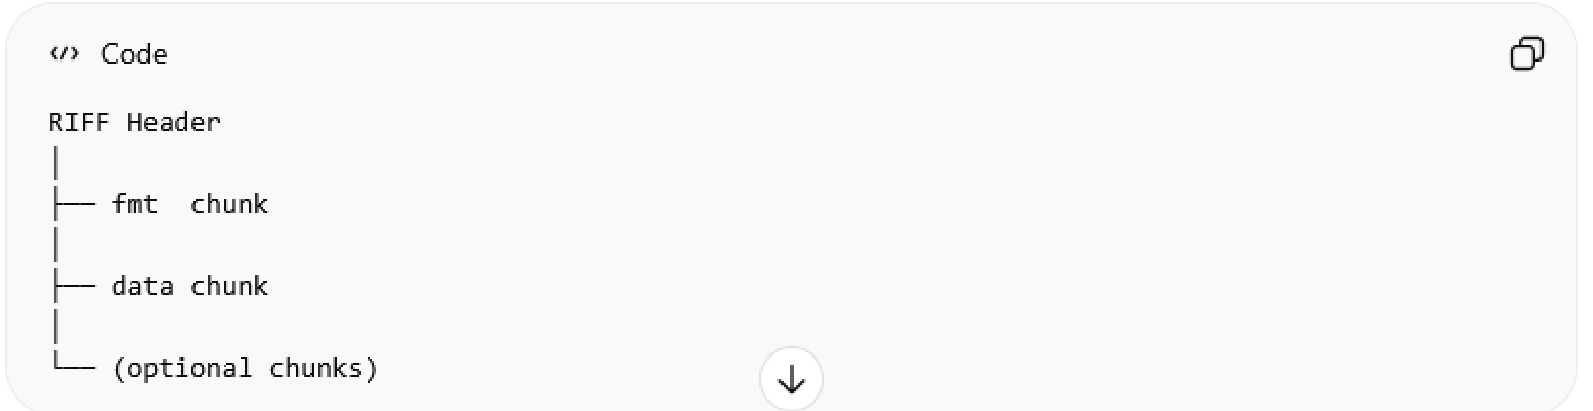
\includegraphics[width=174.30mm,height=112.86mm]{../../images/llm/page_084_img_01.png}%
\end{textblock*}

\end{document}
